%%%%%%%%%%%%%%%%%%%%%%%%%%%%%%%%%%%%%%%%%%%%%%%%%%%%%%%%%%%%%%%%%%
%%%%%%%% ICML 2013 EXAMPLE LATEX SUBMISSION FILE %%%%%%%%%%%%%%%%%
%%%%%%%%%%%%%%%%%%%%%%%%%%%%%%%%%%%%%%%%%%%%%%%%%%%%%%%%%%%%%%%%%%

% Use the following line _only_ if you're still using LaTeX 2.09.
%\documentstyle[icml2013,epsf,natbib]{article}
% If you rely on Latex2e packages, like most moden people use this:
\documentclass{article}

% For figures
\usepackage{graphicx} % more modern
%\usepackage{epsfig} % less modern
% \usepackage{subfigure}
\usepackage{subcaption}
\usepackage{multicol}

% For citations
\usepackage{natbib}

% For algorithms
\usepackage{algorithm}
\usepackage{algorithmic}

% For math
\usepackage{amsmath}
\usepackage{siunitx}

% As of 2011, we use the hyperref package to produce hyperlinks in the
% resulting PDF.  If this breaks your system, please commend out the
% following usepackage line and replace \usepackage{icml2013} with
% \usepackage[nohyperref]{icml2013} above.
\usepackage{hyperref}

% Packages hyperref and algorithmic misbehave sometimes.  We can fix
% this with the following command.
\newcommand{\theHalgorithm}{\arabic{algorithm}}

% Employ the following version of the ``usepackage'' statement for
% submitting the draft version of the paper for review.  This will set
% the note in the first column to ``Under review.  Do not distribute.''
\usepackage{icml2013}
% Employ this version of the ``usepackage'' statement after the paper has
% been accepted, when creating the final version.  This will set the
% note in the first column to ``Proceedings of the...''
% \usepackage[accepted]{icml2013}


% The \icmltitle you define below is probably too long as a header.
% Therefore, a short form for the running title is supplied here:
\icmltitlerunning{6.867: Final Project}

\begin{document}

\twocolumn[
  \icmltitle{6.867: Final Project}

  % % It is OKAY to include author information, even for blind
  % % submissions: the style file will automatically remove it for you
  % % unless you've provided the [accepted] option to the icml2013
  % % package.
  % \icmlauthor{Andrea Li}{liandrea@mit.edu}
  % \icmladdress{Your Fantastic Institute,
  %             314159 Pi St., Palo Alto, CA 94306 USA}
  % \icmlauthor{Tyson Chen}{ytchen33@mit.edu}
  % \icmladdress{Their Fantastic Institute,
  %             27182 Exp St., Toronto, ON M6H 2T1 CANADA}

  % You may provide any keywords that you
  % find helpful for describing your paper; these are used to populate
  % the "keywords" metadata in the PDF but will not be shown in the document

  \vskip 0.3in
]


\section{Introduction}
The NBA is currently one of the most popular sports in the world. Just a few months ago, over 30.8 million viewers tuned into watch Game 7 of the NBA finals between the Cleveland Cavaliers and the Golden State Warriors making it the third most viewed event in the U.S in 2016 (just behind the Super Bowl and the Academy Awards). As a result of this popularity, the betting market for the sport is enormous. NBA commissioner Adam Silver predicted the market to be around 400 billion dollars. 


This report is concerned with exploring a variety of supervised learning techniques in hopes of being able to make predictions of game outcomes that are more accurate than the predictions made by NBA experts who set the betting line for each game. Before diving too deep into the algorithms, models, and predictions, we want to provide a quick overview of the structure of an NBA season as well as the various types of bets you can make in the NBA. 

First, it is important to understand that the NBA is comprised of 30 teams split into two conferences (East and West). These 30 teams will each play 82 games across the regular season meaning that 1230 NBA games are played in total each season. For each game of the season, there are multiple bets that can be made. Below, we will discuss the two most common bets: \\

\textit{a) Win/ Loss:} This is the most basic bet that can be made. The gambler simply picks which team he believes will win the game and if he is correct then he'll win money.

\textit{b) The Spread:} The spread is a bit more advanced than simply win/loss. When a gambler bets against the spread, he either bets that the favorite shall win by more than the spread or that the underdog will lose by less than the spread. Typically, the spread is expressed as a negative number, which signifies the expected margin of victory for the favorite. In order to place a bet against the spread, a gambler generally needs to bet \$110 for the chance to win a \$100 payoff. The amount required for the chance to win \$100 is generally expressed in parentheses.\\
e.g.
Golden State Warriors -7.4 (-110)
Cleveland Cavaliers 7.4 (-110)

The gambling authority generally selects the spread with the goal of splitting the betting money down the line in order to essentially make arbitrage with 0 risk. Due to the fact that the spreads are created in this manner and not with accuracy in mind, we believe that there is definitely room for improvement
\section{Data collection}
For this project, we needed to get gather a great deal of historical NBA game statistics in order to train our models. To collect season data, we primarily used publicly available data from \texttt{http://basketballvalue.com/downloads.php}.
These datasets contained time series data in the form of matchup logs for all NBA games ranging from 2005 to 2012. Matchup logs basically describe the interactions that occur between 5-person units. A new entry is created every time a substitution is made in a game. Through running a python script on these matchup logs, we were able to derive and construct a variety of statistics that would later serve as features. For seasons 2005-2008, the matchup logs were a bit simpler, so we were only able to derive basic statistics including points allowed and points scored. The matchup logs became a bit more advanced in seasons 2008-2011, which allowed us to derive more sophisticated statistics including offensive and defensive rebounds as well as possessions. 

For all seasons, we also constructed a new feature called ELO that is basically a reflection of a teams performance taking into account strength of schedule. What this means is that if two teams possess identical records, one of the teams may actually have a higher ELO score if they had to face stronger competition. In our literature review, this was not a feature that had been incorporated before in machine learning so we were particularly excited about its implications. 

Many of the features generated for training and testing our predictor were derived from this game data. In order to create a general proxy for how strong a team was, we calculated running averages of points allowed, points scored, win rate, ELO, etc. and used these as input features to our classifier. These running averages were initialized to equal numbers for all teams at the beginning of the season and were subsequently updated as more data became available. Because these numbers were arbitrarily initialized to equal at the beginning of the season, however, running averages near the beginning of the season serve as less reliable data points, as outliers can significantly affect the running average.

These statistics were therefore plotted over time throughout the season in order to approximate when the running averages for each of these statistics stabilized to reliable averages. An example graph is given in Figure 1, in which the running average win rate for a given team is plotted over the course of the season.

\begin{figure}[width=\linewidth]
\centering
  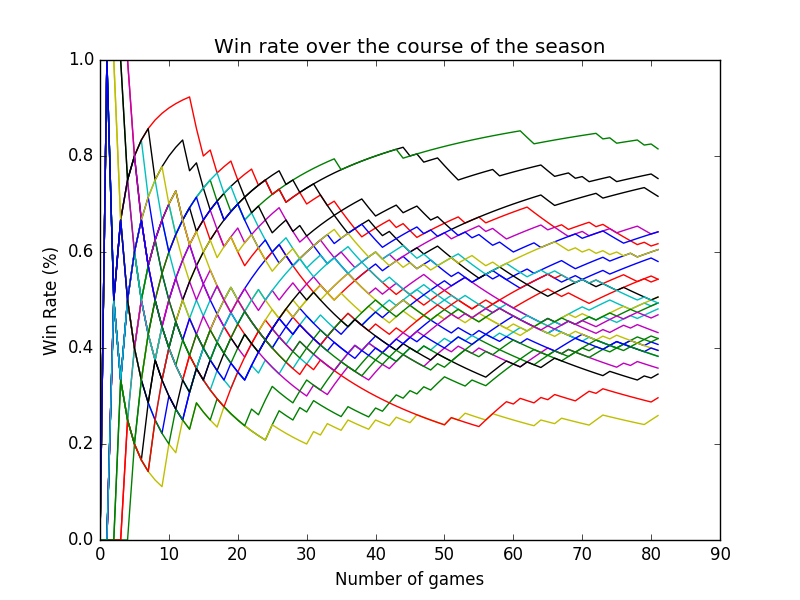
\includegraphics[width=1\linewidth]{code/figures/win_rate.png}
\caption{Win rate over time}
\end{figure}

In general, the running averages of the game data stabilized after approximately each team's twentieth game of the season (around the 1/4th mark of the season). When generating our training, validation, and test sets therefore, we only used data after each team's twentieth game in order to ensure that the features extracted from the data were representative of true team performance.

In order to compare our algorithm and our predicted spreads against Vegas and other betting authorities, we created a scraper to scrape relevant websites with both current and historical spreads. We primarily scraped this information from \texttt{http://www.sportsbookreview.com/betting-odds/} \texttt{nba-basketball/}.

\section{Normalization}
The need for feature normalization arises because our features are on different scales. For example, the average points a team scores every game is around $100$ whereas the average number of offensive rebounds a team gets per game is around $15$. In order to normalize the features we took a Z score approach that centered all the data at $0$ and set the standard deviation to be $1$. 

\section{Linear classifier}
As a baseline, we started with a linear classifier using basic features including running averages of home/away team points scored, points allowed, Elo score, games won, games played, and win rate. Based on the 2006-2007 season, in predicting win/loss (as opposed to the spread of a win/loss), the linear classifier had an accuracy of 64.3\% on training data and 63.3\% on testing data.

After adding further features, such as home court advantage, were added to the model, the linear classifier has an accuracy of 72.3\% on training data and 66.9\% on testing data based on the 2008-2009 season.

We additionally explored the ability of the classifier to predict spreads on games, in which the margin of victory is taken into account instead of a simple win/loss. In this case, the accuracy metric was the absolute value of the difference between the predicted spread and the actual spread. Using basic features on the 2006-2007 season, the average absolute value spread error was 9.31 points for training data and 10.07 points for testing data.

After adding further features, the average absolute value spread error decreased to 8.53 points for training data but increased to 13.60 points for testing data. This would imply that the classifier might be overfitting to the features that are provided as input to the algorithm, which would be expected for more complex architectures but was surprising in the context of the linear classifier explored here.

These results for the performance of the linear classifier are summarized in Table 1.
\begin{table}
  \begin{center}
    \begin{tabular}{ | c | c | c | }
      \hline
                      & Win/Lose Accuracy & Spread Error  \\ \hline
      Basic features  & 63.3\%            & 10.07                 \\ \hline
      Extra features  & 66.9\%            & 13.60                 \\ \hline
    \end{tabular}
  \end{center}
  \caption{Classifier performance on test dataset}
\end{table}

\section{Logistic classifier}


\section{Breakdown of individual work}
The breakdown of work between the two members of the group largely followed that given in the original project proposal. Andrea and Tyson jointly worked on preliminary review of the current techniques and the state of the art. Following this, Tyson was primarily involved in the collection of game data from past seasons, and Andrea created the scraper to collect data on historical spreads put out by various betting organizations on previous games. Andrea explored preliminary models such as linear regression, logistic regression, and regression with various basis functions and various degrees of regularization, and Tyson chiefly explored a neural network approach. As discussed during the project proposal meeting, we decided not to implement a convolutional neural network for this problem, as the architecture did not fit the structure of the problem as closely. We each tested the models we worked on against data test sets and historical spreads, and we split the writing up of the report equally.
>>>>>>> 5fc10a64f5b2fad57f4e7111df70025e3c028062


\end{document}


% This document was modified from the file originally made available by
% Pat Langley and Andrea Danyluk for ICML-2K. This version was
% created by Lise Getoor and Tobias Scheffer, it was slightly modified
% from the 2010 version by Thorsten Joachims & Johannes Fuernkranz,
% slightly modified from the 2009 version by Kiri Wagstaff and
% Sam Roweis's 2008 version, which is slightly modified from
% Prasad Tadepalli's 2007 version which is a lightly
% changed version of the previous year's version by Andrew Moore,
% which was in turn edited from those of Kristian Kersting and
% Codrina Lauth. Alex Smola contributed to the algorithmic style files.
